% Options for packages loaded elsewhere
\PassOptionsToPackage{unicode}{hyperref}
\PassOptionsToPackage{hyphens}{url}
%
\documentclass[
  ignorenonframetext,
  aspectratio=169,
]{beamer}
\usepackage{pgfpages}
\setbeamertemplate{caption}[numbered]
\setbeamertemplate{caption label separator}{: }
\setbeamercolor{caption name}{fg=normal text.fg}
\beamertemplatenavigationsymbolsempty
% Prevent slide breaks in the middle of a paragraph
\widowpenalties 1 10000
\raggedbottom
\setbeamertemplate{part page}{
  \centering
  \begin{beamercolorbox}[sep=16pt,center]{part title}
    \usebeamerfont{part title}\insertpart\par
  \end{beamercolorbox}
}
\setbeamertemplate{section page}{
  \centering
  \begin{beamercolorbox}[sep=12pt,center]{part title}
    \usebeamerfont{section title}\insertsection\par
  \end{beamercolorbox}
}
\setbeamertemplate{subsection page}{
  \centering
  \begin{beamercolorbox}[sep=8pt,center]{part title}
    \usebeamerfont{subsection title}\insertsubsection\par
  \end{beamercolorbox}
}
\AtBeginPart{
  \frame{\partpage}
}
\AtBeginSection{
  \ifbibliography
  \else
    \frame{\sectionpage}
  \fi
}
\AtBeginSubsection{
  \frame{\subsectionpage}
}
\usepackage{amsmath,amssymb}
\usepackage{lmodern}
\usepackage{iftex}
\ifPDFTeX
  \usepackage[T1]{fontenc}
  \usepackage[utf8]{inputenc}
  \usepackage{textcomp} % provide euro and other symbols
\else % if luatex or xetex
  \usepackage{unicode-math}
  \defaultfontfeatures{Scale=MatchLowercase}
  \defaultfontfeatures[\rmfamily]{Ligatures=TeX,Scale=1}
\fi
\usetheme[]{metropolis}
\usecolortheme{seahorse}
% Use upquote if available, for straight quotes in verbatim environments
\IfFileExists{upquote.sty}{\usepackage{upquote}}{}
\IfFileExists{microtype.sty}{% use microtype if available
  \usepackage[]{microtype}
  \UseMicrotypeSet[protrusion]{basicmath} % disable protrusion for tt fonts
}{}
\makeatletter
\@ifundefined{KOMAClassName}{% if non-KOMA class
  \IfFileExists{parskip.sty}{%
    \usepackage{parskip}
  }{% else
    \setlength{\parindent}{0pt}
    \setlength{\parskip}{6pt plus 2pt minus 1pt}}
}{% if KOMA class
  \KOMAoptions{parskip=half}}
\makeatother
\usepackage{xcolor}
\IfFileExists{xurl.sty}{\usepackage{xurl}}{} % add URL line breaks if available
\IfFileExists{bookmark.sty}{\usepackage{bookmark}}{\usepackage{hyperref}}
\hypersetup{
  pdftitle={Session 2},
  pdfauthor={Matt Denwood, Eleftherios Meletis},
  hidelinks,
  pdfcreator={LaTeX via pandoc}}
\urlstyle{same} % disable monospaced font for URLs
\newif\ifbibliography
\usepackage{color}
\usepackage{fancyvrb}
\newcommand{\VerbBar}{|}
\newcommand{\VERB}{\Verb[commandchars=\\\{\}]}
\DefineVerbatimEnvironment{Highlighting}{Verbatim}{commandchars=\\\{\}}
% Add ',fontsize=\small' for more characters per line
\usepackage{framed}
\definecolor{shadecolor}{RGB}{248,248,248}
\newenvironment{Shaded}{\begin{snugshade}}{\end{snugshade}}
\newcommand{\AlertTok}[1]{\textcolor[rgb]{0.94,0.16,0.16}{#1}}
\newcommand{\AnnotationTok}[1]{\textcolor[rgb]{0.56,0.35,0.01}{\textbf{\textit{#1}}}}
\newcommand{\AttributeTok}[1]{\textcolor[rgb]{0.77,0.63,0.00}{#1}}
\newcommand{\BaseNTok}[1]{\textcolor[rgb]{0.00,0.00,0.81}{#1}}
\newcommand{\BuiltInTok}[1]{#1}
\newcommand{\CharTok}[1]{\textcolor[rgb]{0.31,0.60,0.02}{#1}}
\newcommand{\CommentTok}[1]{\textcolor[rgb]{0.56,0.35,0.01}{\textit{#1}}}
\newcommand{\CommentVarTok}[1]{\textcolor[rgb]{0.56,0.35,0.01}{\textbf{\textit{#1}}}}
\newcommand{\ConstantTok}[1]{\textcolor[rgb]{0.00,0.00,0.00}{#1}}
\newcommand{\ControlFlowTok}[1]{\textcolor[rgb]{0.13,0.29,0.53}{\textbf{#1}}}
\newcommand{\DataTypeTok}[1]{\textcolor[rgb]{0.13,0.29,0.53}{#1}}
\newcommand{\DecValTok}[1]{\textcolor[rgb]{0.00,0.00,0.81}{#1}}
\newcommand{\DocumentationTok}[1]{\textcolor[rgb]{0.56,0.35,0.01}{\textbf{\textit{#1}}}}
\newcommand{\ErrorTok}[1]{\textcolor[rgb]{0.64,0.00,0.00}{\textbf{#1}}}
\newcommand{\ExtensionTok}[1]{#1}
\newcommand{\FloatTok}[1]{\textcolor[rgb]{0.00,0.00,0.81}{#1}}
\newcommand{\FunctionTok}[1]{\textcolor[rgb]{0.00,0.00,0.00}{#1}}
\newcommand{\ImportTok}[1]{#1}
\newcommand{\InformationTok}[1]{\textcolor[rgb]{0.56,0.35,0.01}{\textbf{\textit{#1}}}}
\newcommand{\KeywordTok}[1]{\textcolor[rgb]{0.13,0.29,0.53}{\textbf{#1}}}
\newcommand{\NormalTok}[1]{#1}
\newcommand{\OperatorTok}[1]{\textcolor[rgb]{0.81,0.36,0.00}{\textbf{#1}}}
\newcommand{\OtherTok}[1]{\textcolor[rgb]{0.56,0.35,0.01}{#1}}
\newcommand{\PreprocessorTok}[1]{\textcolor[rgb]{0.56,0.35,0.01}{\textit{#1}}}
\newcommand{\RegionMarkerTok}[1]{#1}
\newcommand{\SpecialCharTok}[1]{\textcolor[rgb]{0.00,0.00,0.00}{#1}}
\newcommand{\SpecialStringTok}[1]{\textcolor[rgb]{0.31,0.60,0.02}{#1}}
\newcommand{\StringTok}[1]{\textcolor[rgb]{0.31,0.60,0.02}{#1}}
\newcommand{\VariableTok}[1]{\textcolor[rgb]{0.00,0.00,0.00}{#1}}
\newcommand{\VerbatimStringTok}[1]{\textcolor[rgb]{0.31,0.60,0.02}{#1}}
\newcommand{\WarningTok}[1]{\textcolor[rgb]{0.56,0.35,0.01}{\textbf{\textit{#1}}}}
\usepackage{longtable,booktabs,array}
\usepackage{calc} % for calculating minipage widths
\usepackage{caption}
% Make caption package work with longtable
\makeatletter
\def\fnum@table{\tablename~\thetable}
\makeatother
\usepackage{graphicx}
\makeatletter
\def\maxwidth{\ifdim\Gin@nat@width>\linewidth\linewidth\else\Gin@nat@width\fi}
\def\maxheight{\ifdim\Gin@nat@height>\textheight\textheight\else\Gin@nat@height\fi}
\makeatother
% Scale images if necessary, so that they will not overflow the page
% margins by default, and it is still possible to overwrite the defaults
% using explicit options in \includegraphics[width, height, ...]{}
\setkeys{Gin}{width=\maxwidth,height=\maxheight,keepaspectratio}
% Set default figure placement to htbp
\makeatletter
\def\fps@figure{htbp}
\makeatother
\setlength{\emergencystretch}{3em} % prevent overfull lines
\providecommand{\tightlist}{%
  \setlength{\itemsep}{0pt}\setlength{\parskip}{0pt}}
\setcounter{secnumdepth}{-\maxdimen} % remove section numbering
\makeatletter
\def\verbatim@nolig@list{}
\makeatother


% fontspec requires xelatex which gives problems for me (Matt)
% \usepackage{fontspec}
% % \setmainfont[Ligatures=Historic]{TeX Gyre Pagella}
% \newfontfamily\FiraCode{Fira Code}
% \setmonofont[Contextuals={Alternate}]{Fira Code}
% \newfontfamily\Fontify[Path = ../common/]{Fontify-Regular}
% \else
% \newcommand{\Fontify}{}
% \fi



% \usepackage{fontspec}
% \setmonofont{FiraCode-Regular}[Contextuals=Alternate]
% \usepackage{listings}
% \usepackage[verbatim]{lstfiracode}
% \lstset{style=FiraCodeStyle,basicstyle=\ttfamily}
\usepackage{xspace}
\newcommand{\rlang}[0]{\texttt{R}\xspace}

\newcommand{\rpackage}[1]{\texttt{\{#1\}}}
\newcommand{\dataset}[1]{\textsl{#1}}
% \newcommand{\hotkey}[1]{#1}

% this package is conflicted with the keystroke package.
% \usepackage{statex2}

\usepackage{keystroke}
\usepackage{fvextra}
\fvset{samepage=true}
\fvset{breaklines=true}
\fvset{baselinestretch=1}
%% Adds line numbers to R code chunks in beamer:
% \fvset{numbers=left}
\RecustomVerbatimEnvironment{verbatim}{Verbatim}{breaklines}
%% Controls the font size of R code chunks, but overrides any local settings:
% \fvset{fontsize=\scriptsize}
\usepackage{ccfonts}
\makeatletter
\beamer@ignorenonframefalse
\makeatother

\usepackage{comment}

\ifLuaTeX
  \usepackage{selnolig}  % disable illegal ligatures
\fi

\title{Session 2}
\subtitle{Introduction to Hui-Walter models}
\author{Matt Denwood, Eleftherios Meletis}
\date{2023-06-07}

\begin{document}
\frame{\titlepage}

\begin{frame}{Hui-Walter Model}
\protect\hypertarget{hui-walter-model}{}
\begin{itemize}
\item
  A particular model formulation that was originally designed for
  evaluating diagnostic tests in the absence of a gold standard
\item
  Not necessarily (or originally) Bayesian but often implemented using
  Bayesian MCMC
\item
  But evaluating an imperfect test against another imperfect test is a
  bit like pulling a rabbit out of a hat

  \begin{itemize}
  \tightlist
  \item
    If we don't know the true disease status, how can we estimate
    sensitivity or specificity for either test?
  \end{itemize}
\end{itemize}
\end{frame}

\begin{frame}{The multinomial distribution}
\protect\hypertarget{the-multinomial-distribution}{}
Binomial (always with two possible outcomes):

\scriptsize\includegraphics{Session_2_files/figure-beamer/unnamed-chunk-1-1.pdf}
\normalsize
\end{frame}

\begin{frame}
Multinomial with two possible outcomes:

\scriptsize\includegraphics{Session_2_files/figure-beamer/unnamed-chunk-2-1.pdf}
\normalsize
\end{frame}

\begin{frame}
Multinomial with four possible outcomes:

\scriptsize\includegraphics{Session_2_files/figure-beamer/unnamed-chunk-3-1.pdf}
\normalsize
\end{frame}

\begin{frame}[fragile]{Model Specification}
\protect\hypertarget{model-specification}{}
\scriptsize

\begin{verbatim}
model{
  Tally ~ dmulti(prob, N)
  
  # Test1- Test2-
    prob[1] <- (prev * ((1-se[1])*(1-se[2]))) + ((1-prev) * ((sp[1])*(sp[2])))

  # Test1+ Test2-
    prob[2] <- (prev * ((se[1])*(1-se[2]))) + ((1-prev) * ((1-sp[1])*(sp[2])))

  # Test1- Test2+
    prob[3] <- (prev * ((1-se[1])*(se[2]))) + ((1-prev) * ((sp[1])*(1-sp[2])))
  
  # Test1+ Test2+
    prob[4] <- (prev * ((se[1])*(se[2]))) + ((1-prev) * ((1-sp[1])*(1-sp[2])))
\end{verbatim}

\normalsize
\end{frame}

\begin{frame}[fragile]
\scriptsize

\begin{verbatim}
 

  prev ~ dbeta(1, 1)
  se[1] ~ dbeta(1, 1)
  sp[1] ~ dbeta(1, 1)
  se[2] ~ dbeta(1, 1)
  sp[2] ~ dbeta(1, 1)

  #data# Tally, N
  #monitor# prev, prob, se, sp, deviance
  #inits# prev, se, sp
}
\end{verbatim}

\normalsize
\end{frame}

\begin{frame}[fragile]
\scriptsize

\begin{Shaded}
\begin{Highlighting}[]
\NormalTok{twoXtwo }\OtherTok{\textless{}{-}} \FunctionTok{matrix}\NormalTok{(}\FunctionTok{c}\NormalTok{(}\DecValTok{48}\NormalTok{, }\DecValTok{12}\NormalTok{, }\DecValTok{4}\NormalTok{, }\DecValTok{36}\NormalTok{), }\AttributeTok{ncol=}\DecValTok{2}\NormalTok{, }\AttributeTok{nrow=}\DecValTok{2}\NormalTok{)}
\NormalTok{twoXtwo}
\DocumentationTok{\#\#      [,1] [,2]}
\DocumentationTok{\#\# [1,]   48    4}
\DocumentationTok{\#\# [2,]   12   36}
\end{Highlighting}
\end{Shaded}

\normalsize

\scriptsize

\begin{Shaded}
\begin{Highlighting}[]
\FunctionTok{library}\NormalTok{(}\StringTok{\textquotesingle{}runjags\textquotesingle{}}\NormalTok{)}

\NormalTok{Tally }\OtherTok{\textless{}{-}} \FunctionTok{as.numeric}\NormalTok{(twoXtwo)}
\NormalTok{N }\OtherTok{\textless{}{-}} \FunctionTok{sum}\NormalTok{(Tally)}

\NormalTok{prev }\OtherTok{\textless{}{-}} \FunctionTok{list}\NormalTok{(}\AttributeTok{chain1=}\FloatTok{0.05}\NormalTok{, }\AttributeTok{chain2=}\FloatTok{0.95}\NormalTok{)}
\NormalTok{se }\OtherTok{\textless{}{-}} \FunctionTok{list}\NormalTok{(}\AttributeTok{chain1=}\FunctionTok{c}\NormalTok{(}\FloatTok{0.01}\NormalTok{,}\FloatTok{0.99}\NormalTok{), }\AttributeTok{chain2=}\FunctionTok{c}\NormalTok{(}\FloatTok{0.99}\NormalTok{,}\FloatTok{0.01}\NormalTok{))}
\NormalTok{sp }\OtherTok{\textless{}{-}} \FunctionTok{list}\NormalTok{(}\AttributeTok{chain1=}\FunctionTok{c}\NormalTok{(}\FloatTok{0.01}\NormalTok{,}\FloatTok{0.99}\NormalTok{), }\AttributeTok{chain2=}\FunctionTok{c}\NormalTok{(}\FloatTok{0.99}\NormalTok{,}\FloatTok{0.01}\NormalTok{))}

\NormalTok{results }\OtherTok{\textless{}{-}} \FunctionTok{run.jags}\NormalTok{(}\StringTok{\textquotesingle{}basic\_hw.txt\textquotesingle{}}\NormalTok{, }\AttributeTok{n.chains=}\DecValTok{2}\NormalTok{)}
\end{Highlighting}
\end{Shaded}

\normalsize

{[}Remember to check convergence and effective sample size!{]}
\end{frame}

\begin{frame}[fragile]
\scriptsize

\begin{Shaded}
\begin{Highlighting}[]
\NormalTok{results}
\end{Highlighting}
\end{Shaded}

\normalsize

\scriptsize\includegraphics{Session_2_files/figure-beamer/unnamed-chunk-11-1.pdf}
\includegraphics{Session_2_files/figure-beamer/unnamed-chunk-11-2.pdf}
\includegraphics{Session_2_files/figure-beamer/unnamed-chunk-11-3.pdf}
\includegraphics{Session_2_files/figure-beamer/unnamed-chunk-11-4.pdf}
\includegraphics{Session_2_files/figure-beamer/unnamed-chunk-11-5.pdf}
\includegraphics{Session_2_files/figure-beamer/unnamed-chunk-11-6.pdf}
\includegraphics{Session_2_files/figure-beamer/unnamed-chunk-11-7.pdf}
\includegraphics{Session_2_files/figure-beamer/unnamed-chunk-11-8.pdf}
\includegraphics{Session_2_files/figure-beamer/unnamed-chunk-11-9.pdf}
\includegraphics{Session_2_files/figure-beamer/unnamed-chunk-11-10.pdf}
\includegraphics{Session_2_files/figure-beamer/unnamed-chunk-11-11.pdf}
\normalsize

\scriptsize

\begin{longtable}[]{@{}lrrrrr@{}}
\toprule
& Lower95 & Median & Upper95 & SSeff & psrf \\
\midrule
\endhead
prev & 0.328 & 0.499 & 0.668 & 4250 & 2.288 \\
prob{[}1{]} & 0.367 & 0.462 & 0.558 & 13858 & 1.000 \\
prob{[}2{]} & 0.072 & 0.132 & 0.202 & 14200 & 1.000 \\
prob{[}3{]} & 0.018 & 0.055 & 0.104 & 9602 & 1.000 \\
prob{[}4{]} & 0.255 & 0.343 & 0.438 & 13555 & 1.000 \\
se{[}1{]} & 0.028 & 0.570 & 1.000 & 4564 & 15.155 \\
se{[}2{]} & 0.000 & 0.385 & 0.965 & 4585 & 13.619 \\
sp{[}1{]} & 0.000 & 0.461 & 0.970 & 4527 & 15.261 \\
sp{[}2{]} & 0.036 & 0.581 & 1.000 & 4593 & 13.641 \\
deviance & 12.304 & 15.134 & 21.447 & 8838 & 1.000 \\
\bottomrule
\end{longtable}

\normalsize

\begin{itemize}
\tightlist
\item
  Does anybody spot a problem?
\end{itemize}
\end{frame}

\begin{frame}
\scriptsize\includegraphics{Session_2_files/figure-beamer/unnamed-chunk-13-1.pdf}
\normalsize
\end{frame}

\begin{frame}
\scriptsize\includegraphics{Session_2_files/figure-beamer/unnamed-chunk-14-1.pdf}
\normalsize
\end{frame}

\begin{frame}
\scriptsize\includegraphics{Session_2_files/figure-beamer/unnamed-chunk-15-1.pdf}
\normalsize
\end{frame}

\begin{frame}
\scriptsize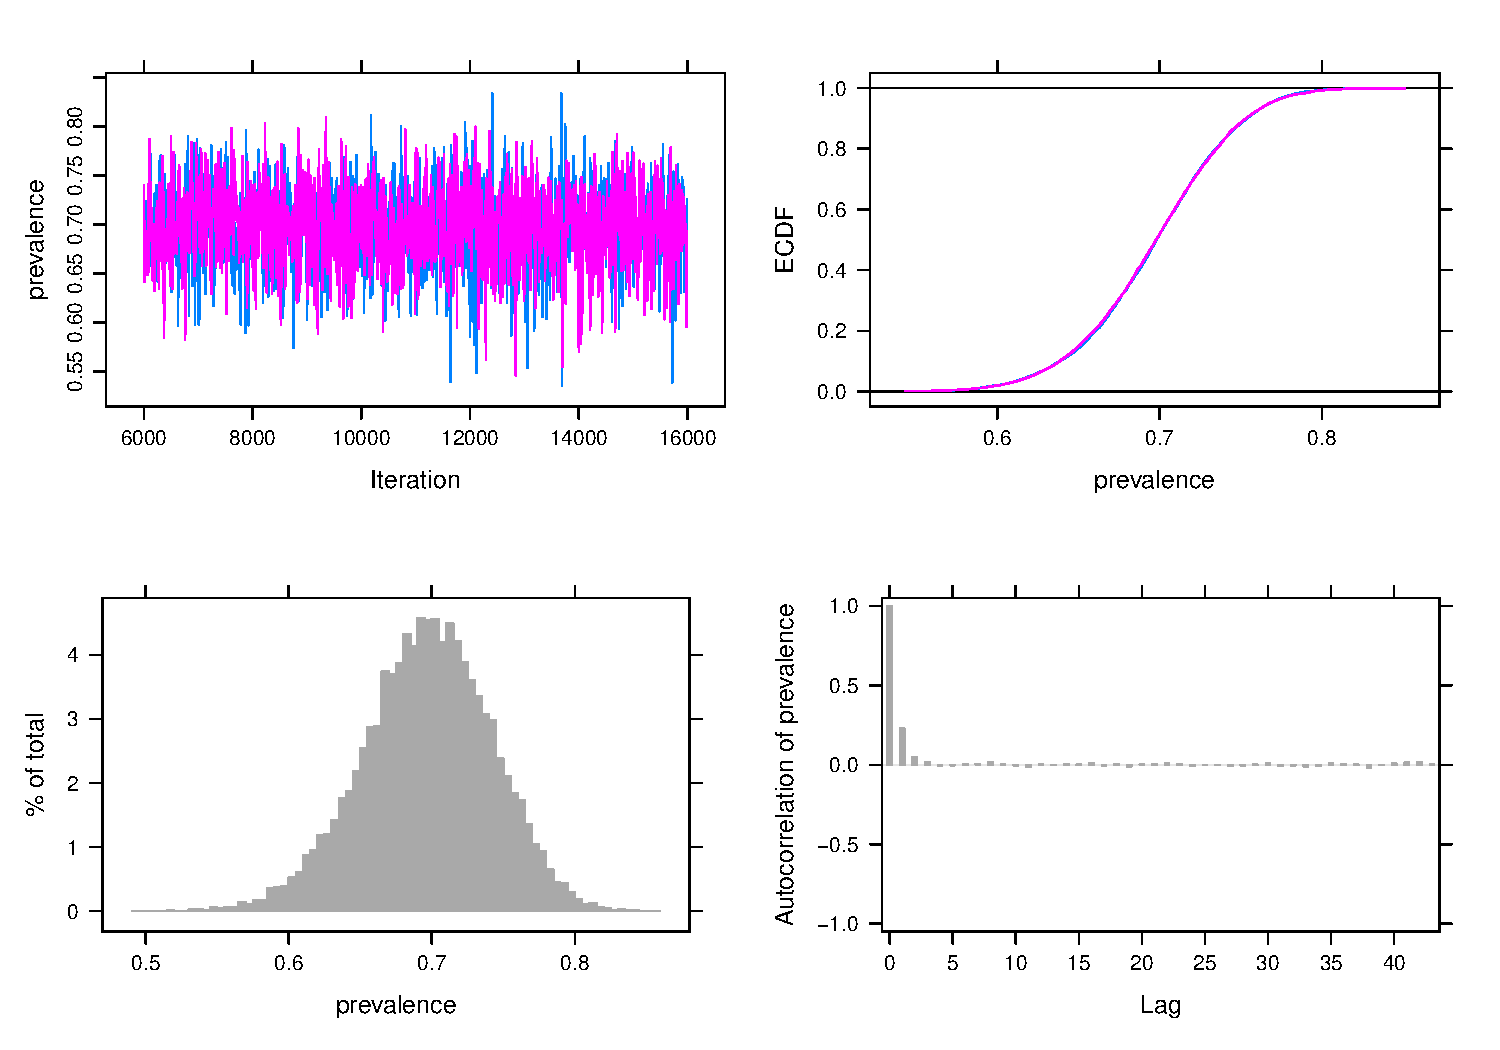
\includegraphics{Session_2_files/figure-beamer/unnamed-chunk-16-1.pdf}
\normalsize
\end{frame}

\begin{frame}
\scriptsize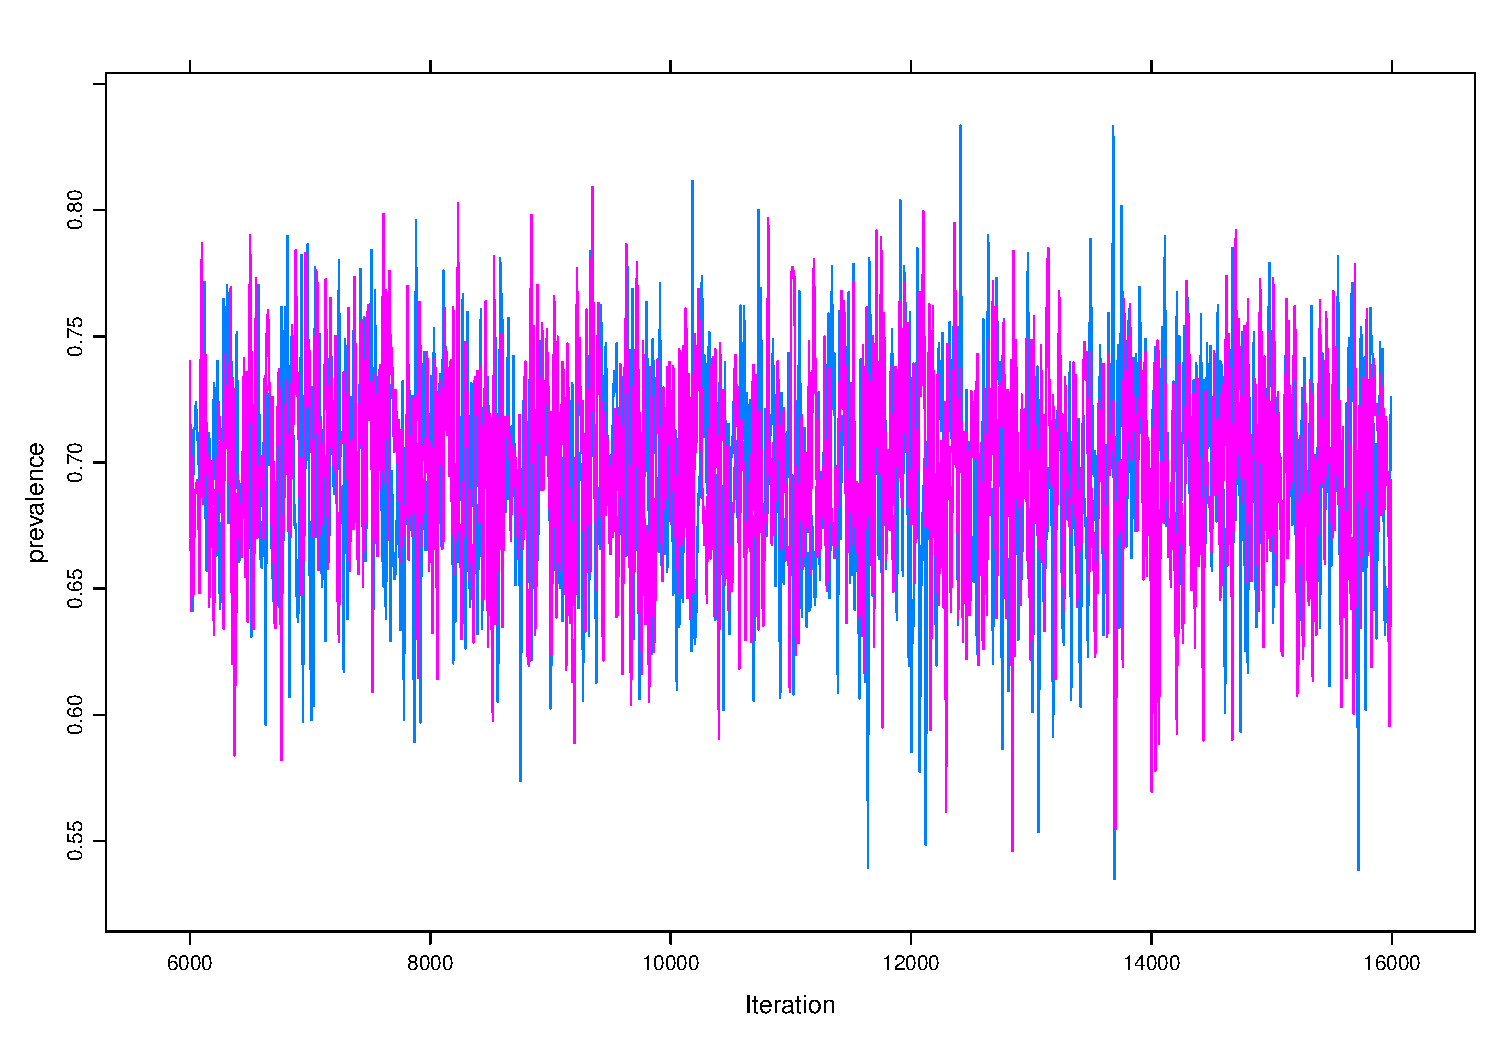
\includegraphics{Session_2_files/figure-beamer/unnamed-chunk-17-1.pdf}
\normalsize
\end{frame}

\begin{frame}
\scriptsize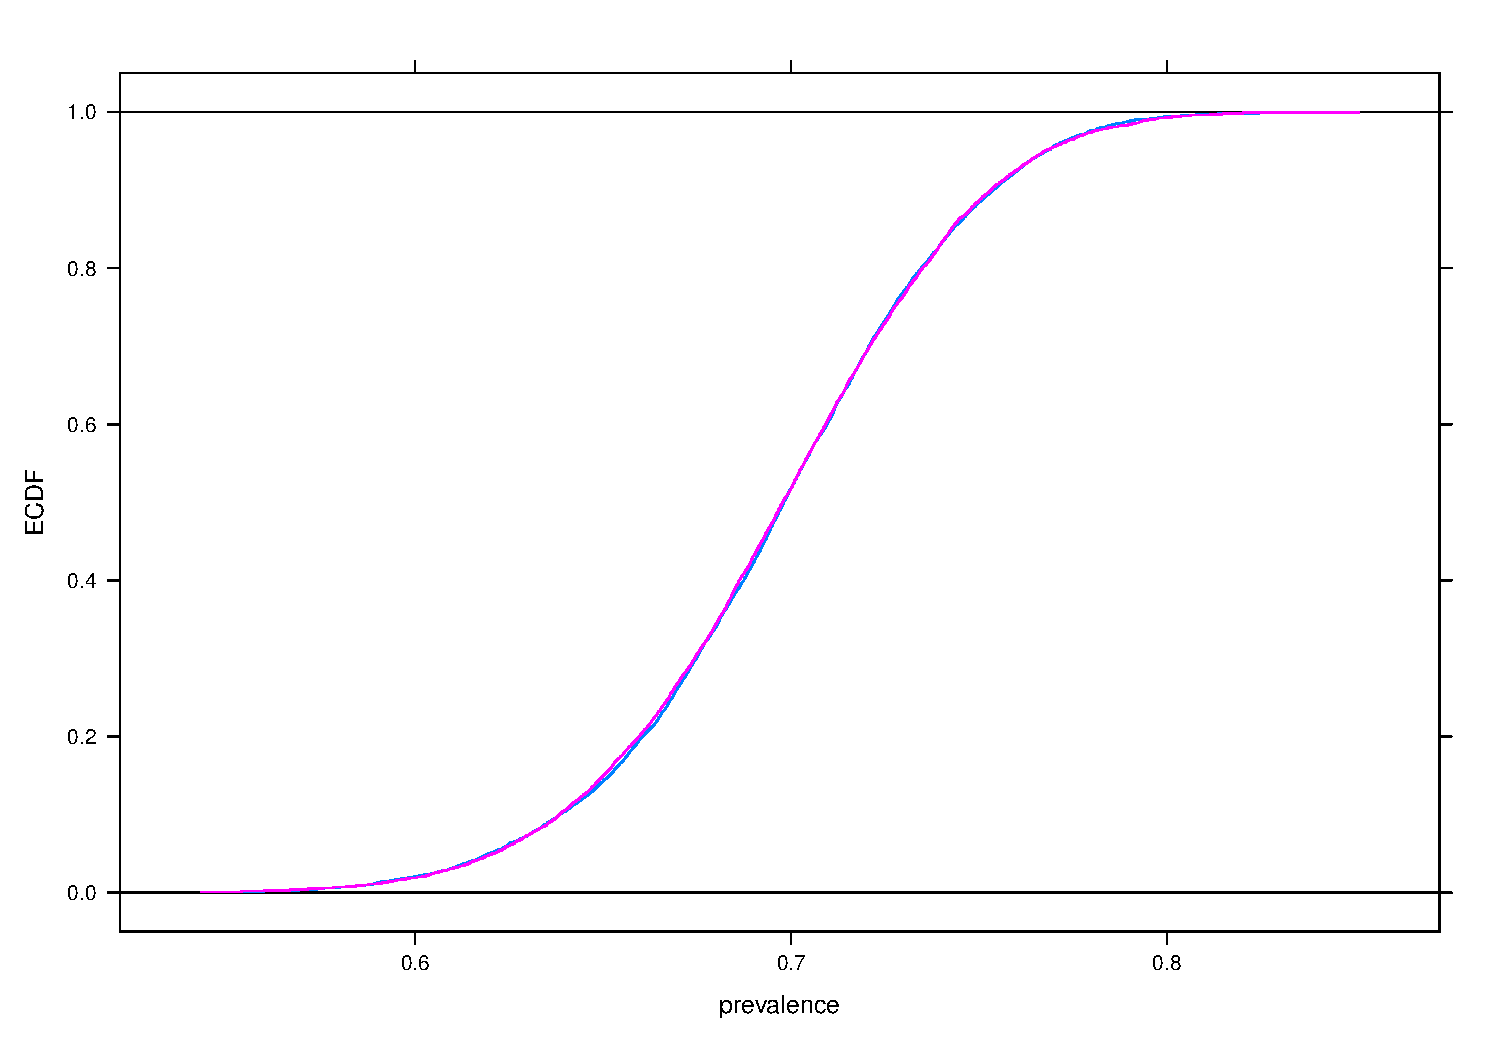
\includegraphics{Session_2_files/figure-beamer/unnamed-chunk-18-1.pdf}
\normalsize
\end{frame}

\begin{frame}[fragile]{Label Switching}
\protect\hypertarget{label-switching}{}
How to interpret a test with Se=0\% and Sp=0\%?

\pause

\begin{itemize}
\tightlist
\item
  The test is perfect - we are just holding it upside down\ldots{}
\end{itemize}

\pause

We can force se+sp \textgreater= 1:

\scriptsize

\begin{Shaded}
\begin{Highlighting}[]
\NormalTok{  se[}\DecValTok{1}\NormalTok{] }\SpecialCharTok{\textasciitilde{}} \FunctionTok{dbeta}\NormalTok{(}\DecValTok{1}\NormalTok{, }\DecValTok{1}\NormalTok{)}
\NormalTok{  sp[}\DecValTok{1}\NormalTok{] }\SpecialCharTok{\textasciitilde{}} \FunctionTok{dbeta}\NormalTok{(}\DecValTok{1}\NormalTok{, }\DecValTok{1}\NormalTok{)}\FunctionTok{T}\NormalTok{(}\DecValTok{1}\SpecialCharTok{{-}}\NormalTok{se[}\DecValTok{1}\NormalTok{], )}
\end{Highlighting}
\end{Shaded}

\normalsize

Or:

\scriptsize

\begin{Shaded}
\begin{Highlighting}[]
\NormalTok{  se[}\DecValTok{1}\NormalTok{] }\SpecialCharTok{\textasciitilde{}} \FunctionTok{dbeta}\NormalTok{(}\DecValTok{1}\NormalTok{, }\DecValTok{1}\NormalTok{)}\FunctionTok{T}\NormalTok{(}\DecValTok{1}\SpecialCharTok{{-}}\NormalTok{sp[}\DecValTok{1}\NormalTok{], )}
\NormalTok{  sp[}\DecValTok{1}\NormalTok{] }\SpecialCharTok{\textasciitilde{}} \FunctionTok{dbeta}\NormalTok{(}\DecValTok{1}\NormalTok{, }\DecValTok{1}\NormalTok{)}
\end{Highlighting}
\end{Shaded}

\normalsize

This allows the test to be useless, but not worse than useless.
\end{frame}

\begin{frame}[fragile]
Alternatively we can have the weakly informative priors:

\scriptsize

\begin{Shaded}
\begin{Highlighting}[]
\NormalTok{  se[}\DecValTok{1}\NormalTok{] }\SpecialCharTok{\textasciitilde{}} \FunctionTok{dbeta}\NormalTok{(}\DecValTok{2}\NormalTok{, }\DecValTok{1}\NormalTok{)}
\NormalTok{  sp[}\DecValTok{1}\NormalTok{] }\SpecialCharTok{\textasciitilde{}} \FunctionTok{dbeta}\NormalTok{(}\DecValTok{2}\NormalTok{, }\DecValTok{1}\NormalTok{)}
\end{Highlighting}
\end{Shaded}

\normalsize

To give the model some information that we expect the test
characteristics to be closer to 100\% than 0\%.

\pause

Or we can use stronger priors for one or both tests.
\end{frame}

\begin{frame}[fragile]{Priors}
\protect\hypertarget{priors}{}
A quick way to see the distribution of a prior:

\scriptsize

\begin{Shaded}
\begin{Highlighting}[]
\FunctionTok{curve}\NormalTok{(}\FunctionTok{dbeta}\NormalTok{(x, }\DecValTok{1}\NormalTok{, }\DecValTok{1}\NormalTok{), }\AttributeTok{from=}\DecValTok{0}\NormalTok{, }\AttributeTok{to=}\DecValTok{1}\NormalTok{)}
\end{Highlighting}
\end{Shaded}

\includegraphics{Session_2_files/figure-beamer/unnamed-chunk-22-1.pdf}

\begin{Shaded}
\begin{Highlighting}[]
\FunctionTok{qbeta}\NormalTok{(}\FunctionTok{c}\NormalTok{(}\FloatTok{0.025}\NormalTok{,}\FloatTok{0.975}\NormalTok{), }\AttributeTok{shape1=}\DecValTok{1}\NormalTok{, }\AttributeTok{shape2=}\DecValTok{1}\NormalTok{)}
\DocumentationTok{\#\# [1] 0.025 0.975}
\end{Highlighting}
\end{Shaded}

\normalsize
\end{frame}

\begin{frame}[fragile]
This was minimally informative, but how does that compare to a weakly
informative prior for e.g.~sensitivity?

\scriptsize

\begin{Shaded}
\begin{Highlighting}[]
\FunctionTok{curve}\NormalTok{(}\FunctionTok{dbeta}\NormalTok{(x, }\DecValTok{2}\NormalTok{, }\DecValTok{1}\NormalTok{), }\AttributeTok{from=}\DecValTok{0}\NormalTok{, }\AttributeTok{to=}\DecValTok{1}\NormalTok{)}
\end{Highlighting}
\end{Shaded}

\includegraphics{Session_2_files/figure-beamer/unnamed-chunk-23-1.pdf}

\begin{Shaded}
\begin{Highlighting}[]
\FunctionTok{qbeta}\NormalTok{(}\FunctionTok{c}\NormalTok{(}\FloatTok{0.025}\NormalTok{,}\FloatTok{0.975}\NormalTok{), }\AttributeTok{shape1=}\DecValTok{2}\NormalTok{, }\AttributeTok{shape2=}\DecValTok{1}\NormalTok{)}
\DocumentationTok{\#\# [1] 0.1581139 0.9874209}
\end{Highlighting}
\end{Shaded}

\normalsize
\end{frame}

\begin{frame}[fragile]
\scriptsize

\begin{Shaded}
\begin{Highlighting}[]
\FunctionTok{qbeta}\NormalTok{(}\FunctionTok{c}\NormalTok{(}\FloatTok{0.025}\NormalTok{,}\FloatTok{0.975}\NormalTok{), }\AttributeTok{shape1=}\DecValTok{2}\NormalTok{, }\AttributeTok{shape2=}\DecValTok{1}\NormalTok{)}
\DocumentationTok{\#\# [1] 0.1581139 0.9874209}
\end{Highlighting}
\end{Shaded}

\normalsize

Or more accurately:

\scriptsize

\begin{Shaded}
\begin{Highlighting}[]
\FunctionTok{library}\NormalTok{(}\StringTok{"TeachingDemos"}\NormalTok{)}
\FunctionTok{hpd}\NormalTok{(qbeta, }\AttributeTok{shape1=}\DecValTok{2}\NormalTok{, }\AttributeTok{shape2=}\DecValTok{1}\NormalTok{)}
\DocumentationTok{\#\# [1] 0.2236068 1.0000000}
\end{Highlighting}
\end{Shaded}

\normalsize

\pause

Credible vs confidence intervals:

\begin{itemize}
\tightlist
\item
  For MCMC these are usually calculated using highest posterior density
  (HPD) intervals
\item
  Therefore there is a difference between:

  \begin{itemize}
  \tightlist
  \item
    \texttt{qbeta(c(0.025,0.975),\ ...)}
  \item
    \texttt{hpd(qbeta,\ ...)}
  \end{itemize}
\item
  Technically HPD intervals are credible intervals\ldots{}
\end{itemize}
\end{frame}

\begin{frame}[fragile]
What about a more informative prior?

\scriptsize

\begin{Shaded}
\begin{Highlighting}[]
\FunctionTok{curve}\NormalTok{(}\FunctionTok{dbeta}\NormalTok{(x, }\DecValTok{20}\NormalTok{, }\DecValTok{2}\NormalTok{), }\AttributeTok{from=}\DecValTok{0}\NormalTok{, }\AttributeTok{to=}\DecValTok{1}\NormalTok{)}
\end{Highlighting}
\end{Shaded}

\includegraphics{Session_2_files/figure-beamer/unnamed-chunk-26-1.pdf}

\begin{Shaded}
\begin{Highlighting}[]
\FunctionTok{qbeta}\NormalTok{(}\FunctionTok{c}\NormalTok{(}\FloatTok{0.025}\NormalTok{,}\FloatTok{0.975}\NormalTok{), }\AttributeTok{shape1=}\DecValTok{20}\NormalTok{, }\AttributeTok{shape2=}\DecValTok{2}\NormalTok{)}
\DocumentationTok{\#\# [1] 0.7618401 0.9882507}
\FunctionTok{hpd}\NormalTok{(qbeta, }\AttributeTok{shape1=}\DecValTok{20}\NormalTok{, }\AttributeTok{shape2=}\DecValTok{2}\NormalTok{)}
\DocumentationTok{\#\# [1] 0.7919691 0.9973994}
\end{Highlighting}
\end{Shaded}

\normalsize
\end{frame}

\begin{frame}{Choosing a prior}
\protect\hypertarget{choosing-a-prior}{}
What we want is e.g.~Beta(20,1)

But typically we have median and 95\% confidence intervals from a paper,
e.g.:

``The median (95\% CI) estimates of the sensitivity and specificity of
the shiny new test were 94\% (92-96\%) and 99\% (97-100\%)
respectively''

\pause

How can we generate a Beta( , ) prior from this?
\end{frame}

\begin{frame}[fragile]{The PriorGen package}
\protect\hypertarget{the-priorgen-package}{}
``The median (95\% CI) estimates of the sensitivity and specificity of
the shiny new test were 94\% (92-96\%) and 99\% (97-100\%)''

\scriptsize

\begin{Shaded}
\begin{Highlighting}[]
\FunctionTok{library}\NormalTok{(}\StringTok{"PriorGen"}\NormalTok{)}
\DocumentationTok{\#\# Loading required package: rootSolve}
\FunctionTok{findbeta}\NormalTok{(}\AttributeTok{themedian =} \FloatTok{0.94}\NormalTok{, }\AttributeTok{percentile.value =} \FloatTok{0.92}\NormalTok{)}
\DocumentationTok{\#\# [1] "The desired Beta distribution that satisfies the specified conditions is: Beta( 429.95 27.76 )"}
\DocumentationTok{\#\# [1] "Here is a plot of the specified distribution."}
\DocumentationTok{\#\# [1] "Descriptive statistics for this distribution are:"}
\DocumentationTok{\#\#    Min. 1st Qu.  Median    Mean 3rd Qu.    Max. }
\DocumentationTok{\#\#  0.8906  0.9322  0.9401  0.9395  0.9474  0.9721 }
\DocumentationTok{\#\# [1] "Verification: The percentile value 0.92 corresponds to the 0.05 th percentile"}
\FunctionTok{hpd}\NormalTok{(qbeta, }\AttributeTok{shape1=}\FloatTok{429.95}\NormalTok{, }\AttributeTok{shape2=}\FloatTok{27.76}\NormalTok{)}
\DocumentationTok{\#\# [1] 0.917172 0.960435}
\end{Highlighting}
\end{Shaded}

\normalsize

\pause

Note: \texttt{themedian} could also be \texttt{themean}
\end{frame}

\begin{frame}[fragile]
\scriptsize

\begin{Shaded}
\begin{Highlighting}[]
\FunctionTok{curve}\NormalTok{(}\FunctionTok{dbeta}\NormalTok{(x, }\AttributeTok{shape1=}\FloatTok{429.95}\NormalTok{, }\AttributeTok{shape2=}\FloatTok{27.76}\NormalTok{))}
\end{Highlighting}
\end{Shaded}

\includegraphics{Session_2_files/figure-beamer/unnamed-chunk-28-1.pdf}
\normalsize
\end{frame}

\begin{frame}[fragile]{Initial values}
\protect\hypertarget{initial-values}{}
Part of the problem before was also that we were specifying extreme
initial values:

\scriptsize

\begin{Shaded}
\begin{Highlighting}[]
\NormalTok{se }\OtherTok{\textless{}{-}} \FunctionTok{list}\NormalTok{(}\AttributeTok{chain1=}\FunctionTok{c}\NormalTok{(}\FloatTok{0.01}\NormalTok{,}\FloatTok{0.99}\NormalTok{), }\AttributeTok{chain2=}\FunctionTok{c}\NormalTok{(}\FloatTok{0.99}\NormalTok{,}\FloatTok{0.01}\NormalTok{))}
\NormalTok{sp }\OtherTok{\textless{}{-}} \FunctionTok{list}\NormalTok{(}\AttributeTok{chain1=}\FunctionTok{c}\NormalTok{(}\FloatTok{0.01}\NormalTok{,}\FloatTok{0.99}\NormalTok{), }\AttributeTok{chain2=}\FunctionTok{c}\NormalTok{(}\FloatTok{0.99}\NormalTok{,}\FloatTok{0.01}\NormalTok{))}
\end{Highlighting}
\end{Shaded}

\normalsize

\pause

Let's change these to:

\scriptsize

\begin{Shaded}
\begin{Highlighting}[]
\NormalTok{se }\OtherTok{\textless{}{-}} \FunctionTok{list}\NormalTok{(}\AttributeTok{chain1=}\FunctionTok{c}\NormalTok{(}\FloatTok{0.5}\NormalTok{,}\FloatTok{0.99}\NormalTok{), }\AttributeTok{chain2=}\FunctionTok{c}\NormalTok{(}\FloatTok{0.99}\NormalTok{,}\FloatTok{0.5}\NormalTok{))}
\NormalTok{sp }\OtherTok{\textless{}{-}} \FunctionTok{list}\NormalTok{(}\AttributeTok{chain1=}\FunctionTok{c}\NormalTok{(}\FloatTok{0.5}\NormalTok{,}\FloatTok{0.99}\NormalTok{), }\AttributeTok{chain2=}\FunctionTok{c}\NormalTok{(}\FloatTok{0.99}\NormalTok{,}\FloatTok{0.5}\NormalTok{))}
\end{Highlighting}
\end{Shaded}

\normalsize
\end{frame}

\begin{frame}[fragile]{Analysing simulated data}
\protect\hypertarget{analysing-simulated-data}{}
This is useful to check that we can recover parameter values!

\scriptsize

\begin{Shaded}
\begin{Highlighting}[]
\CommentTok{\# Set a random seed so that the data are reproducible:}
\FunctionTok{set.seed}\NormalTok{(}\DecValTok{2022{-}09{-}12}\NormalTok{)}

\NormalTok{sensitivity }\OtherTok{\textless{}{-}} \FunctionTok{c}\NormalTok{(}\FloatTok{0.9}\NormalTok{, }\FloatTok{0.6}\NormalTok{)}
\NormalTok{specificity }\OtherTok{\textless{}{-}} \FunctionTok{c}\NormalTok{(}\FloatTok{0.95}\NormalTok{, }\FloatTok{0.9}\NormalTok{)}
\NormalTok{N }\OtherTok{\textless{}{-}} \DecValTok{1000}
\NormalTok{prevalence }\OtherTok{\textless{}{-}} \FloatTok{0.5}

\NormalTok{data }\OtherTok{\textless{}{-}} \FunctionTok{tibble}\NormalTok{(}\AttributeTok{Status =} \FunctionTok{rbinom}\NormalTok{(N, }\DecValTok{1}\NormalTok{, prevalence)) }\SpecialCharTok{\%\textgreater{}\%}
  \FunctionTok{mutate}\NormalTok{(}\AttributeTok{Test1 =} \FunctionTok{rbinom}\NormalTok{(N, }\DecValTok{1}\NormalTok{, sensitivity[}\DecValTok{1}\NormalTok{]}\SpecialCharTok{*}\NormalTok{Status }\SpecialCharTok{+}\NormalTok{ (}\DecValTok{1}\SpecialCharTok{{-}}\NormalTok{specificity[}\DecValTok{1}\NormalTok{])}\SpecialCharTok{*}\NormalTok{(}\DecValTok{1}\SpecialCharTok{{-}}\NormalTok{Status))) }\SpecialCharTok{\%\textgreater{}\%}
  \FunctionTok{mutate}\NormalTok{(}\AttributeTok{Test2 =} \FunctionTok{rbinom}\NormalTok{(N, }\DecValTok{1}\NormalTok{, sensitivity[}\DecValTok{2}\NormalTok{]}\SpecialCharTok{*}\NormalTok{Status }\SpecialCharTok{+}\NormalTok{ (}\DecValTok{1}\SpecialCharTok{{-}}\NormalTok{specificity[}\DecValTok{2}\NormalTok{])}\SpecialCharTok{*}\NormalTok{(}\DecValTok{1}\SpecialCharTok{{-}}\NormalTok{Status)))}

\NormalTok{twoXtwo }\OtherTok{\textless{}{-}} \FunctionTok{with}\NormalTok{(data, }\FunctionTok{table}\NormalTok{(Test1, Test2))}
\NormalTok{Tally }\OtherTok{\textless{}{-}} \FunctionTok{as.numeric}\NormalTok{(twoXtwo)}
\end{Highlighting}
\end{Shaded}

\normalsize

\pause

We know that e.g.~the first test has Sensitivity of 90\% and Specificity
of 95\% - so the model \emph{should} be able to tell us that\ldots{}
\end{frame}

\hypertarget{practical-session-2}{%
\section{Practical Session 2}\label{practical-session-2}}

\begin{frame}[fragile]{Points to consider}
\protect\hypertarget{points-to-consider}{}
\begin{enumerate}
\item
  What is the typical autocorrelation (and therefore effective sample
  size) of Hui-Walter models compared to the simpler models we were
  running earlier? Is there any practical consequence of this?
\item
  How does changing the prior distributions for the se and sp of one
  test affect the inference for the other test parameters?
\end{enumerate}

\begin{comment}


## Exercise 1 {.fragile}

Simulate some data using the code given above (under "Analysing simulated data"), and run it using the following model with truncated Beta(1,1) priors for sensitivity and specificity of both tests:

\scriptsize\normalsize

What are the results?

### Solution 1 {.fragile}

\scriptsize

```r
prev <- list(chain1=0.05, chain2=0.95)
se <- list(chain1=c(0.5,0.99), chain2=c(0.99,0.5))
sp <- list(chain1=c(0.5,0.99), chain2=c(0.99,0.5))

results_tr_1000 <- run.jags('hw_truncated.txt', n.chains=2, sample=10000)

# Note: this is only commented out to save space in the exercise file!
# plot(results_tr_1000)
# check convergence and effective sample size, and then interpret results:
results_tr_1000
```

\normalsize

Note that model does converge, but the effective sample size is NOT high enough with 10000 samples - we need to run for longer to get reliable results:

\scriptsize

```r
results_tr_1000 <- run.jags('hw_truncated.txt', n.chains=2, sample=75000)

# Note: this is only commented out to save space in the exercise file!
# plot(results_tr_1000)
# check convergence and effective sample size, and then interpret results:
results_tr_1000
```

\normalsize

Now we can see that the 95% confidence intervals for prev, se and sp are all quite wide, but at least they do contain the simulation values!

## Exercise 2 {.fragile}

- Find beta distribution priors for:

  * Sensitivity: mean estimate = 0.9 (95% CI: 0.85 - 0.95)
  * Specificity: mean estimate = 0.95 (95%CI: 0.92-0.97)

- Look at these distributions using curve and hpd

- Modify your model from exercise 1 using these priors for test 1 (leave the priors for test 2 unchanged)
  - Make sure to name your new model something different, so that you can easily run it using either set of priors for test 1!

- How does this affect the inference for test 2?


### Solution 2 {.fragile}

Parameters for Sensitivity: mean estimate = 0.9 (95% CI: 0.85 - 0.95):

[Note: this is `themean` rather than `themedian`!]

\scriptsize

```r
PriorGen::findbeta(themean=0.9, percentile.value = 0.85)
hpd(qbeta, shape1=101.43, shape2=11.27)
curve(dbeta(x, 101.43, 11.27), from=0, to=1)
```

\normalsize

Parameters for Specificity: mean estimate = 0.95 (95%CI: 0.92-0.97):

\scriptsize

```r
PriorGen::findbeta(themean=0.95, percentile.value = 0.92)
hpd(qbeta, shape1=162.53, shape2=8.55)
curve(dbeta(x, 162.53, 8.55), from=0, to=1)
```

\normalsize

Here is the updated model using the new prior values:

\scriptsize\normalsize

\scriptsize

```r
results_si_1000 <- run.jags('hw_stronginf.txt', n.chains=2)

# Note: this is only commented out to save space in the exercise file!
# plot(results_si_1000)
# check convergence and effective sample size, and then interpret results:
results_si_1000
```

\normalsize

Note that the 95% confidence intervals are much narrower now, including for test 2!!!  The effective sample size is also much higher because the model is more identifiable (i.e. better behaved).


## Exercise 3 {.fragile}

Now adjust the sample size so that you have N=100, re-simulate the data, and re-run the models with both sets of priors.

  - What do you notice about the results compared to N=1000?
  
Also change the prevalence from 50% to 10% or 90%

  - How does this affect your ability to estimate the sensitivity and specificity of test 2 (using strong priors for test 1)?

### Solution 3 {.fragile}

We can change the sample size like so:

\scriptsize

```r
# Set a random seed so that the data are reproducible:
set.seed(2022-09-12)

se <- c(0.9, 0.6)
sp <- c(0.95, 0.9)
N <- 100
prevalence <- 0.5

data <- tibble(Status = rbinom(N, 1, prevalence)) %>%
  mutate(Test1 = rbinom(N, 1, se[1]*Status + (1-sp[1])*(1-Status))) %>%
  mutate(Test2 = rbinom(N, 1, se[2]*Status + (1-sp[2])*(1-Status)))

twoXtwo <- with(data, table(Test1, Test2))
Tally <- as.numeric(twoXtwo)

results_si_100 <- run.jags('hw_stronginf.txt', n.chains=2)
results_tr_100 <- run.jags('hw_truncated.txt', n.chains=2)

# Remember to check convergence!
# plot(results_si_100)
# plot(results_tr_100)

# Comparison to larger dataset:
results_si_100
results_tr_100
results_si_1000
results_tr_1000
```

\normalsize

Note that the posteriors have wider confidence intervals for the smaller dataset, particularly with the weakly informative (truncated) prior for test 1.

With a very low prevalence:

\scriptsize

```r
# Set a random seed so that the data are reproducible:
set.seed(2022-09-12)

se <- c(0.9, 0.6)
sp <- c(0.95, 0.9)
N <- 1000
prevalence <- 0.1

data <- tibble(Status = rbinom(N, 1, prevalence)) %>%
  mutate(Test1 = rbinom(N, 1, se[1]*Status + (1-sp[1])*(1-Status))) %>%
  mutate(Test2 = rbinom(N, 1, se[2]*Status + (1-sp[2])*(1-Status)))

twoXtwo <- with(data, table(Test1, Test2))
Tally <- as.numeric(twoXtwo)

results_lowprev <- run.jags('hw_stronginf.txt', n.chains=2)

# Remember to check convergence!
# plot(results_lowprev)

results_lowprev
```

\normalsize

The specificity for test 2 is well estimated but the sensitivity has large confidence intervals.  This is because there are relatively few true positive samples from which sensitivity can be estimated.  The opposite is true with high prevalence i.e. it is harder to estimate specificity.


## Optional exercise A {.fragile}

Adapt the model so that you can specify the 'hyper-priors' of the sensitivity and specificity for both tests as data

Now pretend that the manufacturer of the test told you that Test 1 actually has these characteristics:

  * Sensitivity = 0.95 (95% CI: 0.92 - 0.98)
  * Specificity = 0.999 (95%CI: 0.99 - 1.00)

Re-estimate the values you would need to use for the priors

Now run your adapted model using these values instead (using the original dataset with N=1000 and prevalence=0.5)
  - What effect does the change to Test 1 priors have on the posterior for Test 2?
  - Other than comparing to the simulation parameters (which you would not know in real life!) is there any way that you can tell the priors for test 1 are not realistic?
  
### Solution A {.fragile}

We need two additional parameters where we fix the value in R and pass that value into JAGS as data:

\scriptsize\normalsize

\scriptsize

```r
# Set a random seed so that the data are reproducible:
set.seed(2022-09-12)

se <- c(0.9, 0.6)
sp <- c(0.95, 0.9)
N <- 1000
prevalence <- 0.5

data <- tibble(Status = rbinom(N, 1, prevalence)) %>%
  mutate(Test1 = rbinom(N, 1, se[1]*Status + (1-sp[1])*(1-Status))) %>%
  mutate(Test2 = rbinom(N, 1, se[2]*Status + (1-sp[2])*(1-Status)))

twoXtwo <- with(data, table(Test1, Test2))
Tally <- as.numeric(twoXtwo)

# Additional data needed for the adapted model:
(se_prior <- matrix(1, ncol=2, nrow=2))
(sp_prior <- matrix(1, ncol=2, nrow=2))

# New priors from the manufacturer:
#  * Sensitivity = 0.95 (95% CI: 0.92 - 0.98)
#  * Specificity = 0.999 (95%CI: 0.99 - 1.00)

PriorGen::findbeta(themedian = 0.95, percentile=0.95, percentile.value = 0.92)
se_prior[1,] <- c(101.43, 11.27)
TeachingDemos::hpd(qbeta, shape1=se_prior[1,1], shape2=se_prior[1,2])

PriorGen::findbeta(themedian = 0.999, percentile=0.95, percentile.value = 0.99)
sp_prior[1,] <- c(162.53, 8.55)
TeachingDemos::hpd(qbeta, shape1=sp_prior[1,1], shape2=sp_prior[1,2])

# Now our hyper-prior parameters look like:
se_prior
sp_prior

# Re-run the model with these prirs:
results_manufacturer <- run.jags('hw_hyperprior.txt', n.chains=2)

# Remember to check convergence!
# plot(results_manufacturer)

results_manufacturer
results_si_1000
```

\normalsize

Compared to the earlier results (results_si_1000), the sensitivity and specificty of test 1 are estimated to be higher, but the sensitivity of test 2 is estimated to be lower. In fact, the 95% CI for specificity of test 2 no longer contains the true simulation value (0.9). Having too much confidence in the performance of one test will always make all of the other tests look worse! So remember to carefully assess the studies on which you base your priors:  if these come from laboratory validation exercises (which typically involve spiked samples with extremely high concentrations of the target vs completely clean/sterile negative controls) then this may not be a realistic estimation of the sensitivity or specificity in the field.

In general the best way to assess the effect of your priors is by sensitivity analysis:  change the priors slightly (for example make them less informative) and see if your posterior changes substantially.  In this case we can see that the stronger priors for test 1 move the estimates for test 2 substantially, so we would have to be extremely sure that these priors are correct in order to believe the model results.

\end{comment}
\end{frame}

\begin{frame}[fragile]{Summary}
\protect\hypertarget{summary}{}
\begin{itemize}
\tightlist
\item
  Hui-Walter models are seemingly magical, but:

  \begin{itemize}
  \tightlist
  \item
    They typically exhibit high autocorrelation
  \item
    They may not converge, particularly with 1 population (see later!)
  \item
    Need a larger sample for the same effective sample size
  \end{itemize}
\item
  More informative priors for one test will

  \begin{itemize}
  \tightlist
  \item
    Improve identifiability of the model
  \item
    Affect the posterior inference for the other test!
  \end{itemize}
\end{itemize}
\end{frame}

\end{document}
